\documentclass[12pt,a4paper,oneside]{article}
\usepackage{graphicx}
\usepackage{titlepic}
\usepackage[utf8]{inputenc}
\usepackage[left=1.1in,right=1.1in, top=1in, bottom= 1in]{geometry}
\usepackage{amsfonts}
\usepackage{amssymb}
\usepackage{amsmath}
\usepackage{fancyhdr}
\usepackage[hidelinks]{hyperref}
\usepackage{listings}
\usepackage{xcolor}
\usepackage[export]{adjustbox}

\definecolor{codegreen}{rgb}{0,0.6,0}
\definecolor{codegray}{rgb}{0.5,0.5,0.5}
\definecolor{codepurple}{rgb}{0.58,0,0.82}
\definecolor{backcolour}{rgb}{0.95,0.95,0.92}

\lstdefinestyle{mystyle}{
    backgroundcolor=\color{backcolour},   
    commentstyle=\color{codegreen},
    keywordstyle=\color{magenta},
    numberstyle=\tiny\color{codegray},
    stringstyle=\color{codepurple},
    basicstyle=\ttfamily\footnotesize,
    breakatwhitespace=false,         
    breaklines=true,                 
    captionpos=b,                    
    keepspaces=true,                 
    numbers=left,                    
    numbersep=5pt,                  
    showspaces=false,                
    showstringspaces=false,
    showtabs=false,                  
    tabsize=2
}

\lstset{style=mystyle}
\usepackage{etoolbox}
\usepackage[nottoc]{tocbibind}
\usepackage{appendix}
\usepackage{multicol}
\usepackage{leftidx}
\graphicspath{{figures/}}
\usepackage{ragged2e}
\usepackage{mathtools}
\usepackage{units}
\usepackage{float}
\usepackage{subcaption}
\usepackage{commath}


\usepackage{amsthm}
 
\theoremstyle{definition}
\newtheorem{definition}{Definition}[section]

\newtheorem{theorem}{Theorem}

\usepackage[none]{hyphenat} % Avoids to go out of margin

\usepackage{subfiles}
\usepackage{imakeidx}
% --------------------------------------------- %

\title{Final Project}	                                    % Title
\author{Mattia Aquilina 1921153 \\\\ Francesco Fortunato 1848527    \\\\ Cristian Santaroni 1800659 }	
% Authors separated by \\
\date{\today}									    % Date

% Font size of figure smaller than normal size:
\usepackage{caption}
\captionsetup[figure]{font=small}
%\captionsetup[table]{font=small}

%\usepackage{setspace} % double spacing
\linespread{1.2}

\makeatletter
\let\thetitle\@title
\let\theauthor\@author
\let\thedate\@date
\makeatother


\begin{document}


\begin{titlepage}
	\centering
    \vspace*{0.5 cm}
    
\includegraphics[scale = 0.75]{figures/SapienzaLogo.pdf}\\[1.0 cm]	% University Logo

    \vspace*{-0.4cm}
    \textsc{\large Department of DIAG}\\[2.0 cm]	% Department Name
    \vspace*{1cm}

    { \fontsize{20.74pt}{18.5pt}\selectfont\bfseries \thetitle \par } % Title

    \vspace*{0.25cm}
    \textsc{\Large The Last Survivor}\\[0.2 cm] % Course Name
    \textsc{Interactive Graphics Course}\\[0.3 cm] % Course Name

    \vspace*{2.6cm}
	\begin{minipage}{0.4\textwidth} % 0.4
		\begin{flushleft} \large
			\textbf{Professor:}\\
			Marco Schaerf\\
		\end{flushleft}
	\end{minipage}~
	\begin{minipage}{0.3\textwidth} %0.4
		\begin{flushright} \large
		\begin{minipage}{1\textwidth}
		\begin{flushleft} \large
			\textbf{Students:} \\
			\theauthor
        \end{flushleft}
        \end{minipage}
		\end{flushright}
	\end{minipage}\\[3.85 cm]

    \vspace{2cm}
    \rule{\linewidth}{0.2 mm} \\[0.3 cm]
    \vspace*{-0.2cm}
    Academic Year 2022/2023
\end{titlepage}

\tableofcontents
\newpage

\section{Introduction}

The Last Survivor is a survival arcade game. A player must survive endless waves of attacking zombies, earning points from killing or damaging zombies. These points can be used to purchase weapons. Zombies spawn in the player-area of the map in specific fixed spot.
Zombies become higher numbers upon the completion of each round.
The game ends when the player has been taken down by the zombies. 


\section{Technologies}
Our game project utilizes a variety of technologies to create immersive and interactive gaming experience. Here are the key technologies employed in the development of our game:
\paragraph{Babylon.js}
We chose \textbf{Babylon.js} as the core engine for our game. Babylon.js provides a robust set of tools and functionalities for rendering 3D graphics, handling animations, managing scenes, and implementing physics simulations. 
\paragraph{HTML5 and CSS}
To create the user interface and layout of our game, we utilized standard web technologies like \textbf{HTML5} and \textbf{CSS}. 

\paragraph{Sketchfab}
We relied on the \textbf{Sketchfab} platform to source high-quality 3D models for various game elements, such as player weapons and enemy characters.

\paragraph{WebGL}
Babylon.js utilizes \textbf{WebGL} (Web Graphics Library) as the underlying technology for rendering hardware-accelerated 3D graphics in the browser.

\paragraph{Blender} 
Blender is a free and open-source 3D computer graphics software. It has been widely used for many aspect of the design like creation of the navmesh or hierachical model inspection.

\paragraph{Yuka}
Yuka provides a basic game entity concept and classes for state-driven and goal-driven agent design.
Graph classes, search algorithms and a navigation mesh implementation enables advanced path finding.
\section{Game Logic and Design}

In this section we will be analyzing how the game evolves and how each interaction has been designed.

\subsection{Game flow}

As briefly explained in the intro, the game consists in round being that follows up until the player dies. At each round a unit manager spawns a fixed number of zombies (depending on the difficulty) and keeps track of their actions. As the goal of the player is to survive, his primarily objective is to kill all the zombies that spawn in each round. For each hit, and every time the player kills a zombie he gain money that can be invested in the lucky box in order to find better weapons (later on each weapon will be discussed). Every time a round is completed a pause timer starts showing the reaming time for the next round to start. Lastly, at start every round (including the first one) ammo boxes are spawned, or replenished, across the map.

\subsection{Enemy Logic}
The main goal of the enemies i.e. the zombies, is to chase the player and try to kill him. In order to do that they have to find the bast path to reach the player, but of course avoiding the obstacles. Each zombie can be hit by the player and receive an amount of damage based on the gun that the player is using. This amount of damage is computed using the health remaining and amount of damage received. Whenever it is hit it release a spray of blood used like an hitmarker to make more easy understanding if the zombie is hit. As soon as we progress completing a round, a new number of zombies based on a multiplier, will spawn again allowing to earn new money.
If the difficult is changed the zombies will have more health and so they became more hard to kill.

The class ``\textbf{Enemy}'' contains all the functions and all the attributes needed to design the zombie, like references to the various components of the model itself, some references to the player, the movement speed and its health. When the zombie is spawned it initializes a constructor to load the needed attributes and the position of the zombie are chosen from an array of position.
The correct spawning is handled by the function \textbf{getPosition()} which project the mesh to the ground.
Then it has to find a path , it is done thanks to the function ``\textbf{findPathTo()}''. This function is based on the position of the player and zombie and  it is called based on a time received from ``getDeltaTime()''. This function is strongly related to a right computation of the navMesh(chapter 5.1.1) and for this reason using the Yuka library was possible to read it correctly. Whenever the mesh of the zombie is hit by the player, computing the health reduction is based on the gun type with which we are playing( different weapons can do different damages), this is managed by the function ``\textbf{takeDamage()}''. \\


\subsection{Player Logic}

For player logic, we refers in managing all the interactions between the user and the player. The most import part is probably the input, that for the movement, is dealt using babylon's camera methods, while all the other types of input are dealt in a special class called Player. This class realizes a finite state machine, where we keep track of the current state of the user, and check the legality of each transition using and apposite function. Each status is always associated with an animation that plays and locks temporally the possibility to change the state until it finishes. Once the animation elapse, the player will return in a idle state. The player states are:
\begin{enumerate}
    \item Idle;
    \item Reloading, the player is reloading the weapon. At end of the animation a new magazine is loaded in the current weapon. This is status is reachable only if the user has shoot at least one round and has enough stacked ammunition;
    \item Shooting, the player is shooting with his weapon. Each time this state is on, a ray is cast to realize the gun shot with pew function.
\end{enumerate}

The player classes manages also the health of the player, setting timeouts so the player can recover his health, and stores the current weapon that the user is holding. 


\subsubsection{Weapons}\label{weapons}

We have three different weapons in our game, each one associated wih a different class. But let's go step by step.

The main class, the ``\textbf{Weapon}'' one, serves as the base class for all weapons in the game. It contains essential attributes and methods for managing weapon behavior, such as fire rate, damage, ammo levels, and the reload animation. Additionally, it includes properties for loading and playing sound effects associated with shooting and reloading. The weapon classes include the general ``Weapon'' class and three subclasses: ``\textbf{Sniper}'', ``\textbf{Pistol}'', and ``\textbf{Assault}''.
The ``\textbf{Pistol}'' class, a subclass of ``Weapon'', represents the pistol weapon in the game. Here are the details of the Pistol:

\begin{itemize}
    \item Damage: 25
    \item Ammo Level: 10
    \item Stocked Ammo: 30
    \item Current Ammo: 10
\end{itemize}

The ``\textbf{Assault Rifle}'' is a versatile and reliable weapon designed for rapid-fire engagements. Here are the details of the Assault Rifle:

\begin{itemize}
    \item Damage: 20
    \item Ammo Level: 30
    \item Stocked Ammo: 60
    \item Current Ammo: 30
\end{itemize}

The ``\textbf{Sniper Rifle}'' is a high-powered weapon designed for long-range precision shooting. It offers incredible damage output and accuracy for eliminating targets from a distance. Here are the details of the Sniper Rifle:

\begin{itemize}
    \item Damage: 400
    \item Ammo Level: 5
    \item Stocked Ammo: 15
    \item Current Ammo: 5
\end{itemize}

\subsection{Settings and Game modes}
This section focuses on the settings implemented in our game project, aiming to allow customizability and optimize the user gameplay experience. So, let's go deeper into the functionalities of the settings menu.

\begin{itemize}
    \item \textbf{Difficulty}: The difficulty setting allows players to adjust the game's level of challenge in order to customize their gameplay experience. The available options are \textbf{Easy}, \textbf{Normal}, and \textbf{Insane}. Each difficulty level affects various aspects of the game, such as enemy strength, weapon recoil, or overall game difficulty:
    \begin{itemize}
        \item \textbf{Easy}: Almost no weapon recoil, weak enemies.
        \item \textbf{Normal}: Recoil slightly increased, stronger enemies.
        \item \textbf{Insane}: The recoil is very realistic, by aiming is difficult to hit enemies. Also zombies are much powered and higher hp.
    \end{itemize}
    \item \textbf{Time}: The time setting provides the ability to switch between day and night mode. Changing the time setting alter the game's visual ambiance and lighting conditions. 
    \begin{itemize}
        \item \textbf{Day mode} represents a brighter environment with more visibility;
        \item \textbf{Night mode} creates a darker and more challenging atmosphere, with a spotlight that can be toggled to help to see better.
    \end{itemize}
    \item \textbf{Motion Blur}: The motion blur setting controls the presence or absence of motion blur effects. 
    \item \textbf{Sensitivity}: The sensitivity setting allows the player to adjust the camera or mouse sensitivity. Higher sensitivity values make the camera or mouse movement more responsive to input, resulting in faster rotations or cursor movements. Lower sensitivity values provide finer control, reducing the speed and intensity of camera or mouse movements.
    \item \textbf{Volume}: The volume setting enables the player to control the audio volume within the game. Adjusting the volume slider allows the player to increase or decrease the sound effects, background music, and other audio elements in the game. 
    \item \textbf{Save}, \textbf{Reset}, and \textbf{Exit} \textbf{Buttons}: 
    \begin{itemize}
        \item The save button allows the player to save the chosen settings and apply them to the game.
        \item The reset button reverts all settings to their default values, effectively resetting any modifications made by the player.
        \item The exit button allows the player to exit the settings menu and return to the main menu.
    \end{itemize}

    
\end{itemize}


\section{Models and Animations}

\subsection{Player's weapon}
The weapon system in our game project encompasses different classes representing specific types of weapons. To achieve this, we have utilized the Sketchfab platform to download high-quality weapon models. The weapon classes include the general ``Weapon'' class and three subclasses: ``\textbf{Sniper}'', ``\textbf{Pistol}'', and ``\textbf{Assault}''. In this section, we will provide an overview of the weapon models and animations.

As stated in \ref{weapons}, the ``\textbf{Weapon}'' class serves as the base class for all weapons in the game.

All of the weapon models are loaded using the \textit{loadMesh} method inherited from the ``Weapon'' class. The method loads the mesh from the specified file location and positions it in the scene.

The weapon models are constructed using a \textbf{hierarchical structure}, which allows for the manipulation of its various components. The model consists of multiple parts, such as the pistol body, magazine, hand controls, and arm. These parts are represented as nodes in the hierarchy and are positioned and rotated relative to their parent nodes.

\begin{figure*}
\begin{multicols}{3}
    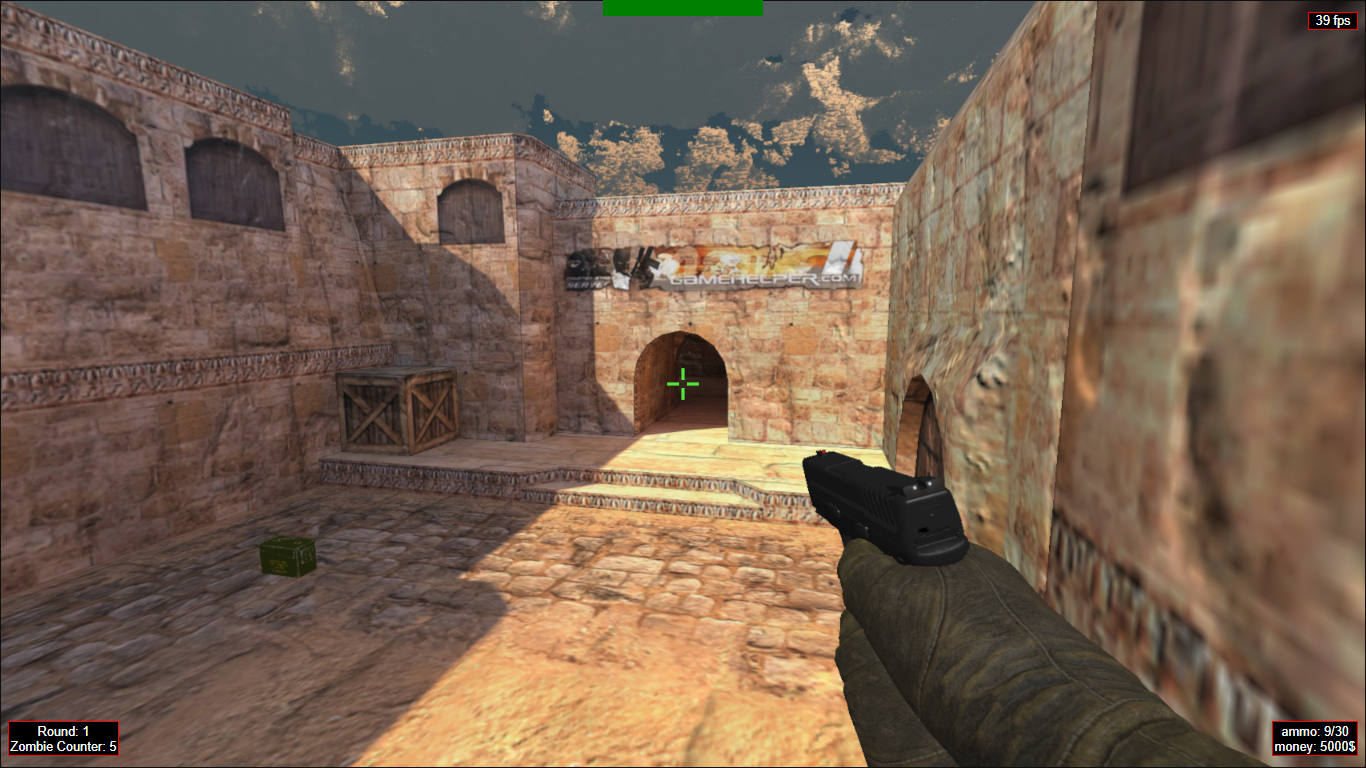
\includegraphics[width=\linewidth]{figures/pistol.png}\par 
    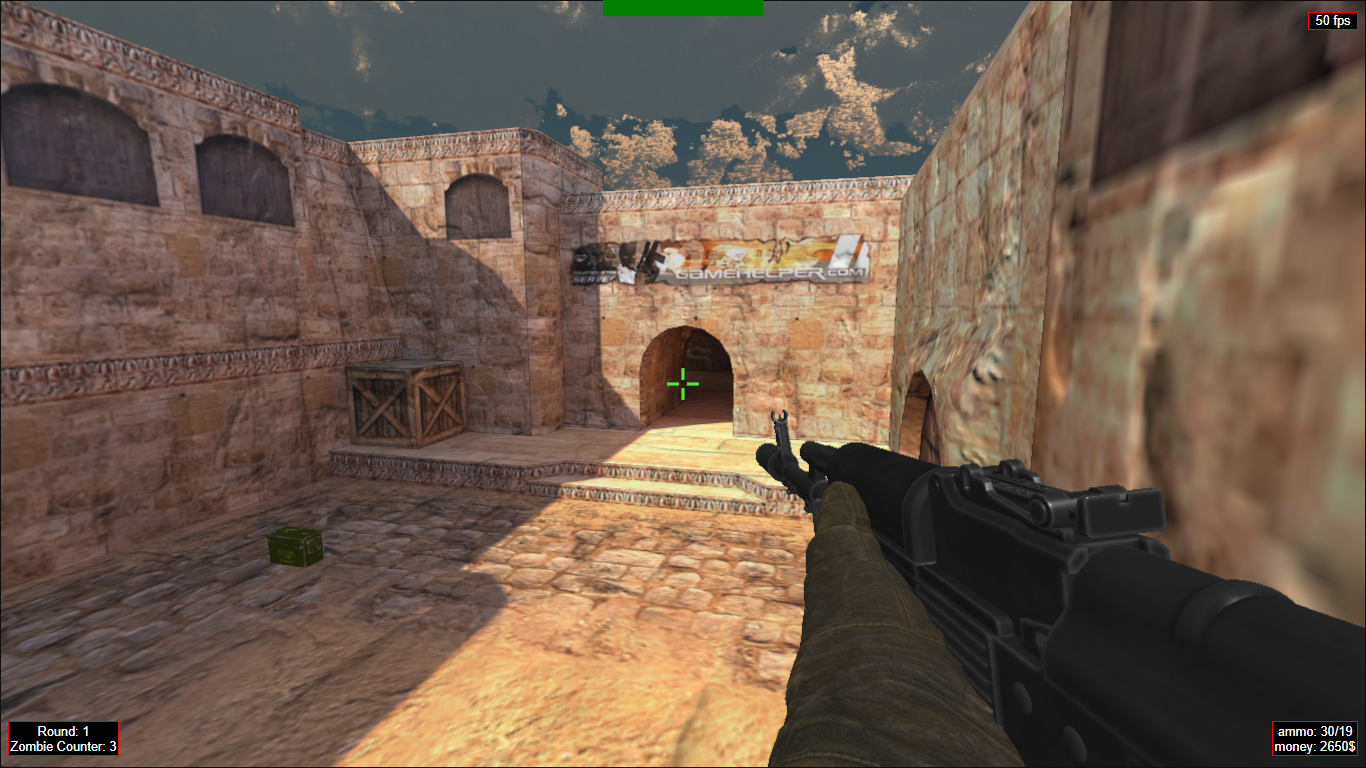
\includegraphics[width=\linewidth]{figures/assault.png}\par 
    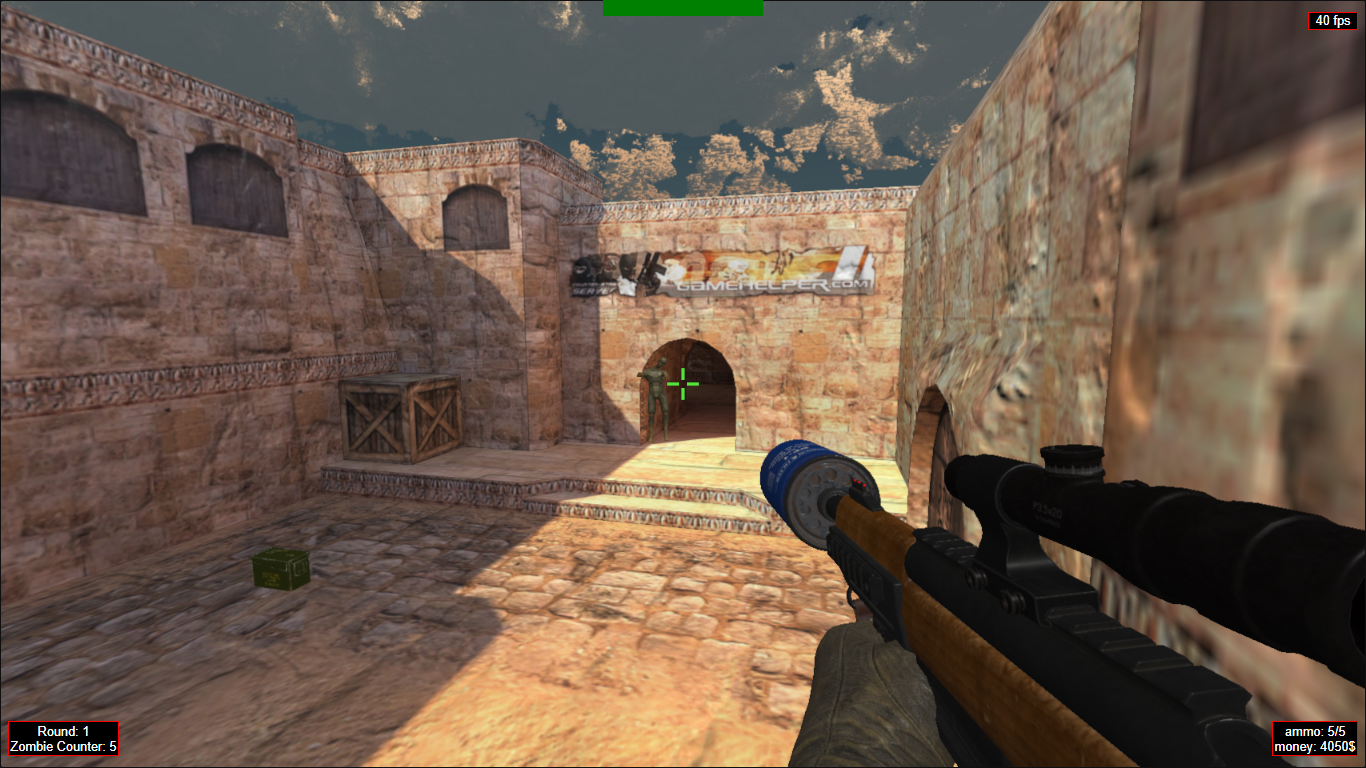
\includegraphics[width=\linewidth]{figures/sniper.png}\par 
    \end{multicols}
\caption{The three weapons: pistol, assault and sniper}
\end{figure*}

\paragraph{Animation} All of these classes define various animation sequences for shooting, reloading and aiming. These animations are loaded using the LoadShootAnimations method. The animations are created using the BABYLON.Animation class and they are assigned to the corresponding components of the pistol model. These animations exploit the \textbf{hierarchical structure} of the weapon models. The hierarchy allows us to control different parts of the model independently, by animating specific components while keeping others static. The animation frames are defined using the \textbf{keyframe technique}, specifying the frame number and the corresponding property values for each frame to each part of the model. Keyframes are essential in defining the animation behavior of the pistol model. They represent specific positions and rotations of the components at different frames of the animation. For the \textbf{pistol}, for example, the code includes keyframes for the position and rotation of the following components:

\begin{itemize}
    \item Magazine (Pmag)
    \item Pistol Body (PBody)
    \item Left Hand Control (IK\_Hand\_Cntrl\_L)
    \item Right Hand Control (IK\_Hand\_Cntrl\_R)
\end{itemize}

For the sniper and the assault rifle, similar components are used to build the animation.
To orchestrate the different components' movements, animation groups are created. These groups contain multiple animations that target specific components. Each weapon has three animation groups: ``\textbf{fire}'', ``\textbf{aim}'' and ``\textbf{reload}''. The reload animation is shared among the weapons and is the same for each of them: it's simply a rotation along the x-axis. The fire animation group controls the firing sequence of the specific weapon, while the aim animation group handles the aiming animation of each weapon. The fire animation simulate the recoil and movement during firing. The aim animation group animates the rifle for aiming. It includes keyframe animations for position and rotation to provide a realistic aiming experience.

To enhance the realism and the gameplay experience, we have also implemented \textbf{camera animations} for the player's aim and shoot actions.

When the player aims their weapon, we smoothly transition the camera's \textbf{field of view} (\textbf{FOV}) to provide a zoomed-in effect. The \textit{animateAimFOV} method handles this animation. It takes the target FOV as a parameter and calculates the intermediate FOV values between the current FOV and the target FOV over a specified number of frames. We use the BABYLON.Animation class to create a smooth zoomed-in and out animation for the camera's FOV property. The animation is played using the this.scene.beginAnimation method.

During the shoot action, we also apply a camera rotation along the x-axis animation to simulate \textbf{recoil}. The \textit{pew} method triggers the shooting effects and rotates the camera. For the Sniper weapon, we rotate the camera by a higher amount. For other weapons, the rotation depends on the difficulty level. We use the \textit{rotateCamera} method to animate the camera rotation. Similar to the FOV animation, we create a rotation animation using the BABYLON.Animation class and apply it to the camera. For these last two animations, the BABYLON.Scalar.Lerp function is used to interpolate between initial and target values over a specified frame count. 

\begin{figure*}
\begin{multicols}{3}
    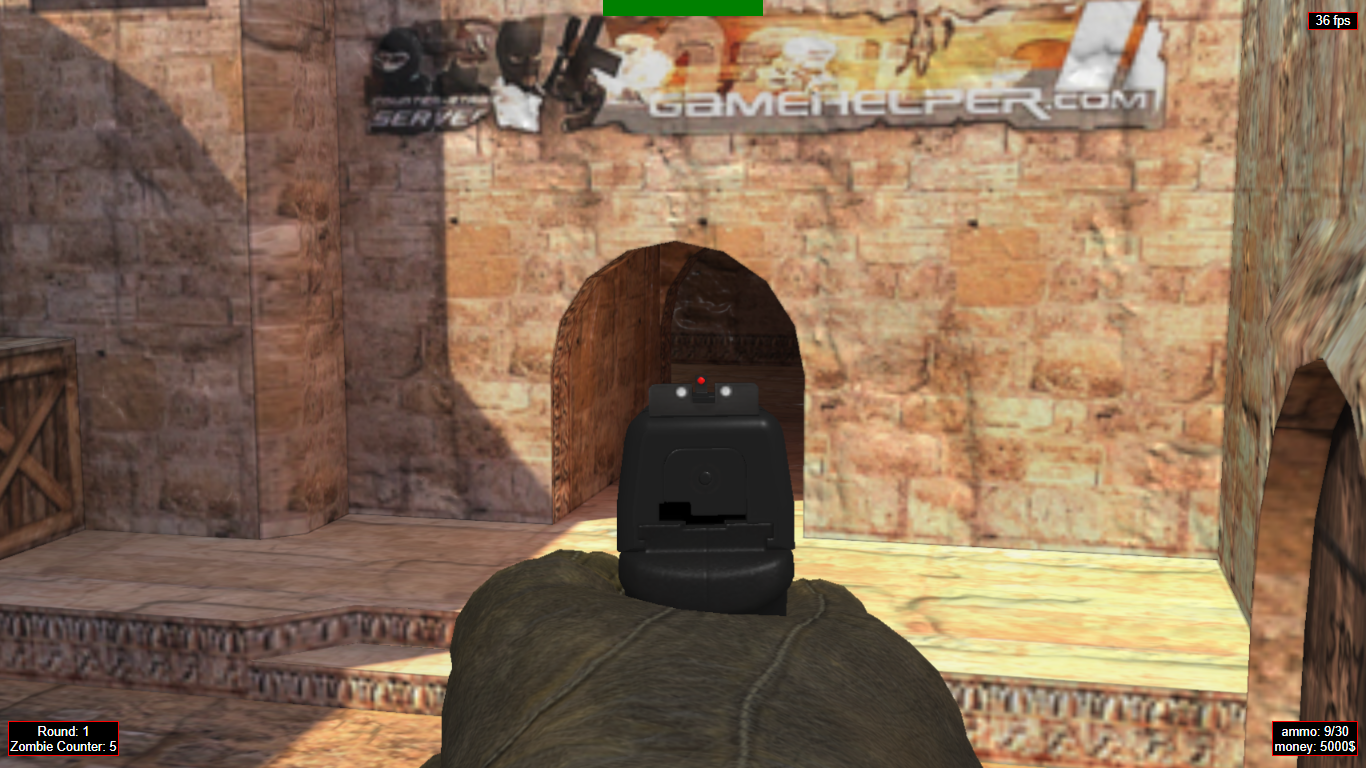
\includegraphics[width=\linewidth]{figures/pistol_aim.png}\par 
    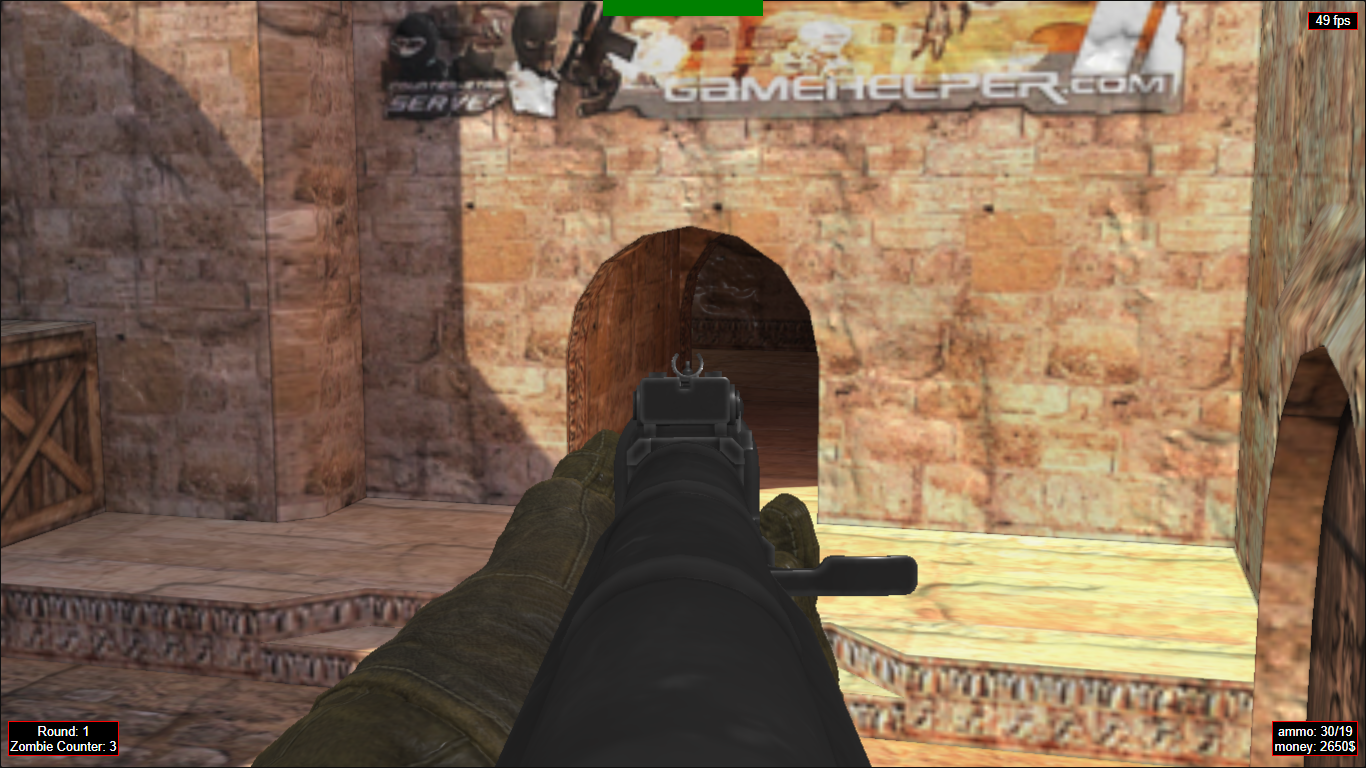
\includegraphics[width=\linewidth]{figures/assault_aim.png}\par 
    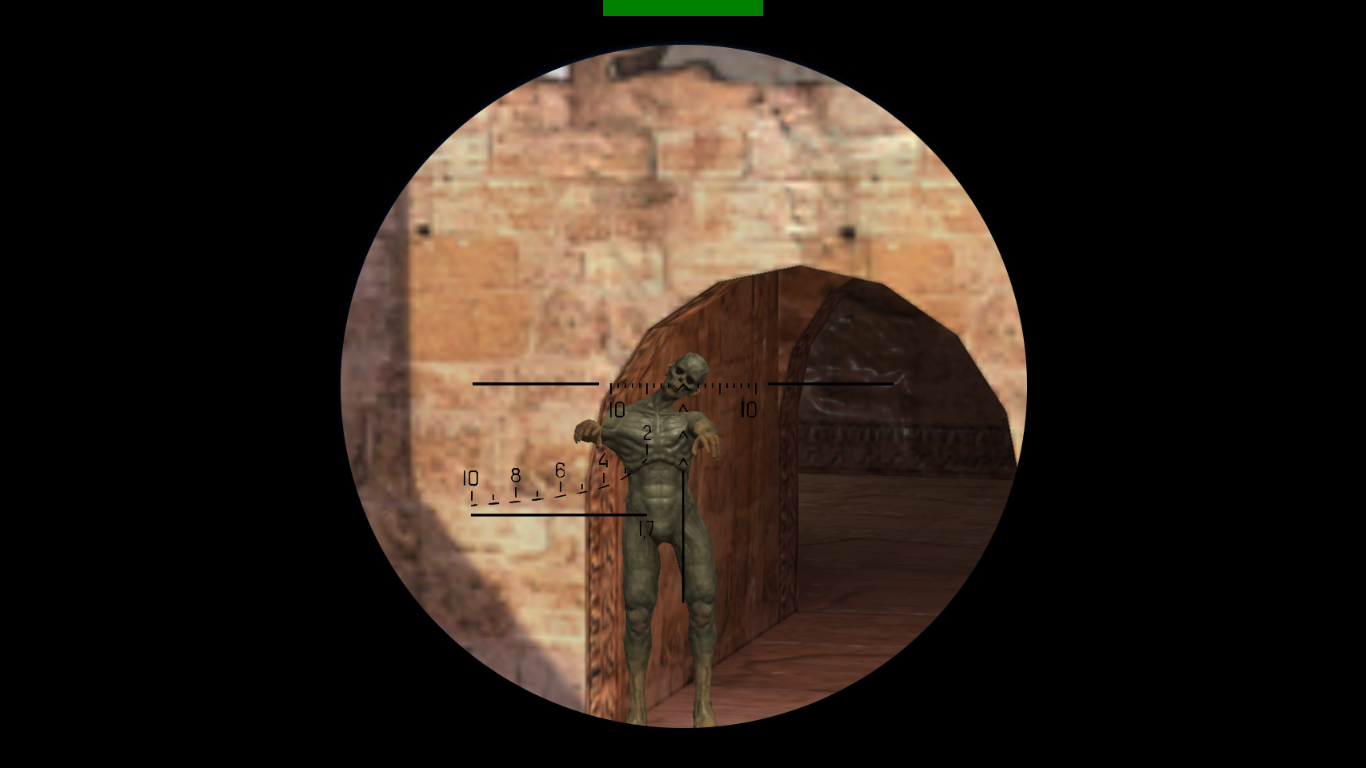
\includegraphics[width=\linewidth]{figures/sniper_aim.png}\par 
    \end{multicols}
\caption{Aiming with pistol, assault rifle and sniper rifle}
\end{figure*}


\subsection{Enemy}
The model representing the enemy is a zombie, it is a complex 3D hierarchical model composed by many joints, also this is imported from sketchfab. The joints choosen to be animated were :

\begin{multicols}{2}
\begin{itemize}
    \item Neck
    \item Left arm
    \item Right arm
    \item Left leg
    \item Right leg    
\end{itemize}\par 
    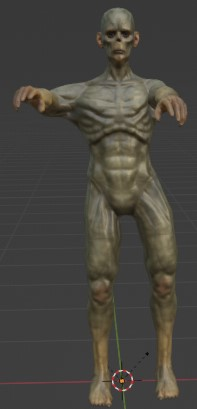
\includegraphics[width=.2\textwidth,center]{figures/zombie.jpg} \par 
    \end{multicols}
This model is composed by 3 different textures: one for the color texture,one for the bump texture and one for the specular color.
\paragraph{Animation}  The animation is based on the movement of the pieces described above and it is handled by the function ``\textbf{WalkingAnimation()}''.The number of key frames is not the same for all the pieces because in order to realize a smoother animation, for some of them like the legs and the arm were needed more keyframes. The animation can be divided into 3 subsequent animations: one to rotate, from left to right, the neck(the joint for the head ) , one performing the walking translating the left and right legs and the last one rotating the right arm to perform an attack.


\subsection{Lucky box and Ammo box}
Ammobox and Luckybox are two important features in our game project that improve the gameplay experience. Let's discuss each of them in detail:

\paragraph{Ammobox} The Ammobox is an interactable object in the game that provides the player with additional ammunition for their weapon. When the player's character comes into contact with the Ammobox, the game logic triggers an action to update the player's ammunition count.
In the implemented code, the player's interaction with the Ammobox is detected through collision detection. When the player character collides with the Ammobox, the game logic increments the player's stocked ammunition based on the ammo level specified for the player's weapon. Additionally, a visual feedback message is displayed to inform the player that they have obtained additional ammo. Finally, after a collision detection, the Ammobox is disposed.
The Ammobox feature adds strategic depth to the gameplay by allowing players to replenish their ammunition during combat. It encourages resource management and decision-making, as players need to strategically engage with Ammoboxes to ensure they have an adequate supply of ammunition for their weapon. Seven ammobox are spawned at each round.

\paragraph{Luckybox} The Luckybox is another interactable object in the game that offers a unique gameplay opportunity for the player. When the player has a sufficient ($950\$$) amount of in-game currency (represented by the ``money'' variable), a particle system is triggered and the users can choose to interact with the Luckybox and spend their money to receive a (potentially) new weapon.
In the provided code, the player's interaction with the Luckybox is initiated by pressing the ``F'' key on the keyboard. If the player has enough money and the Luckybox is interactable, the game logic triggers the \textbf{animation} opening of the Luckybox and deducts the corresponding amount of money from the player's currency. After that another animation is triggered so that the Luckybox is closed again.
The Luckybox feature adds an element of chance and excitement to the game. Players have the opportunity to potentially change the weapon in-game and this can positively impact their gameplay experience. 

\begin{figure*}
\begin{multicols}{2}
    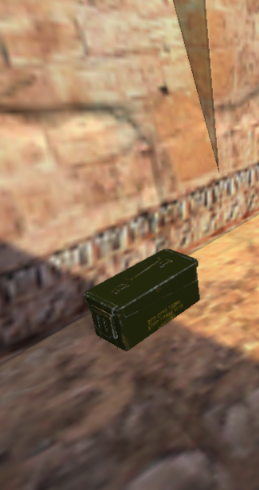
\includegraphics[height=\linewidth]{figures/Ammobox.png}\par 
    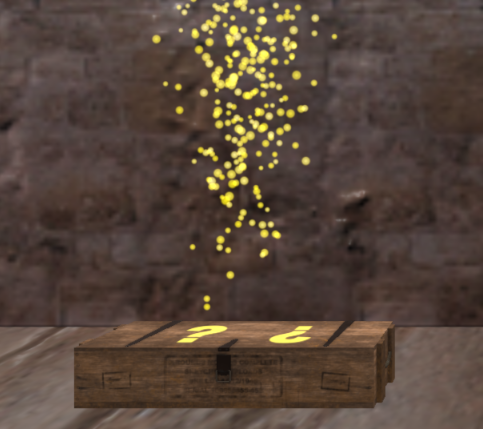
\includegraphics[width=\linewidth]{figures/Luckybox.png}\par 
    \end{multicols}
\caption{Interactable items: ammobox on the left, luckybox on the right}
\end{figure*}

\section{Environment}

\subsection{The map}
\begin{figure}[H]
    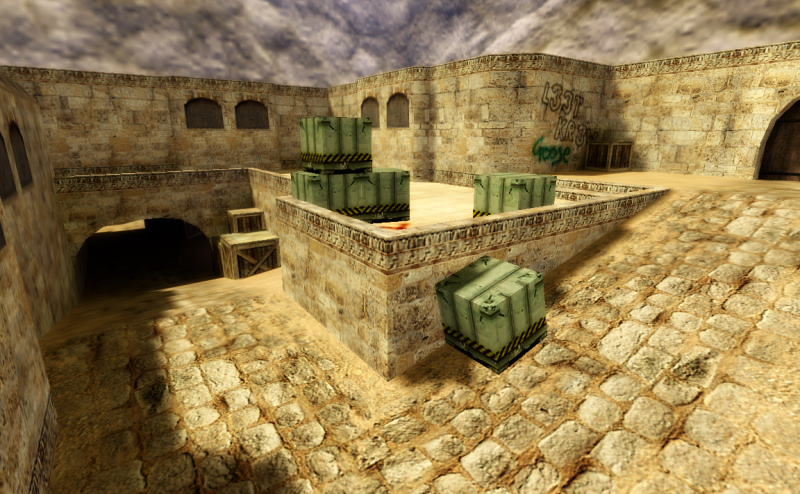
\includegraphics[width=.6\textwidth,center]{figures/dust_2.jpg}
    \caption{The Map}
\end{figure}
The map is set in a Middle Eastern town,the central structure contains more distinct architecture elements and  there are signs of recent conflict littered around the map. The map is a 3D model imported from sketchfab, composed by different pieces.


\subsubsection{Navmesh}
A navigation mesh is a collection of two-dimensional convex polygons (a polygon mesh) that define which areas of the map are traversable by agents.Pathfinding within one of these polygons can be done trivially in a straight line because the polygon is convex and traversable. Pathfinding between polygons in the mesh is done thank to the Yuka library which performs an A* algorithm to find the path. The navigation mesh is computed through blender , and in order to make as precise as possible the path finding was necessary to regulate the precision with which the agent can move between the obstacles of the map.

\subsection{Lights and Textures}

To achieve a more realistic effects in the scene an emispheric light and spotlight have been added to the scene. In particular, the emispheric light realizes the day and night effect. The spotlight is attachted to the camera and can be seen during the night mode, where it helps the player spotting the zombies. 

For what concern the textures, we firstly added a skybox to the environment that displays a sunny and cloudy sky. The sky box turns black, thanks to the fog, during the night mode. Lastly, in order to make the map work with lights, specific shaders with bumps texture have been created using blender.

\subsection{Post processing and particle system}

\paragraph{Post-processing} The main post processing effect is the motion blur. It can be activated or deactivated through settings of the main menu and it applies to the scene a blurring effect. 
\paragraph{Particle system}
The particle system is used to add the effect of the blood to zombies and to highlight the lucky box. When the zombie is hit by the player it generates a bloody effect that is implemented through a particle system where each particle is affected by the gravity in order to give it a real effect of blooding. For the lucky box the particle system is different because it is not affected by the gravity and it acts like a fountain , for this reason was necessary to add the emission rate  to dictate the amount of spray. The lucky box is not always  highlighted, it depends on the amount of money that the player has. If it is greater than 950 \$ a particle system will appear above the lucky box otherwise there will be nothing.  


\subsection{Audio}
Audio plays an important role in improving the immersive experience of the game. Here's a brief overview of the audio elements in the project:
\begin{itemize}
    \item Sounds effects are attached to enemies mesh and are triggered  when they:
    \begin{itemize}
        \item Attack: Audio effects are used to indicate enemy attacks adding intensity and alerting the player to incoming threats;
        \item Hit: Audio feedback is provided when enemies are hit, providing a sense of impact;
        \item Dead.
    \end{itemize}
    \item Weapon:
    \begin{itemize}
        \item Shooting: The weapon emits audio sounds when shooting, simulating the realistic effect of gunfire and adding to the overall immersion of firing. A different audio effect is given for each weapon.
        \item Reloading: Also the reloading process is accompanied by audio effects, signaling the player's ammunition replenishment and maintaining the flow of gameplay.
    \end{itemize}
    \item Toggling the Torch;
    \item Main Menu and In-Game Sounds.

\end{itemize}
\end{document}